% !TEX TS-program = pdflatex
% !TEX encoding = UTF-8 Unicode

\documentclass[hyperref={colorlinks = true, linkcolor=blue},8pt]{beamer}

\usepackage[backend=biber, style=nature, doi=false, url=false, isbn=false ]{biblatex}  

% Macro and bibliography redefinitions to linkify titles, not put links directly in bibliography
\newbibmacro{string+doiurlisbn}[1]{%
  \iffieldundef{doi}{%
    \iffieldundef{url}{%
      \iffieldundef{isbn}{%
        \iffieldundef{issn}{%
          #1%
        }{%
          \href{http://books.google.com/books?vid=ISSN\thefield{issn}}{#1}%
        }%
      }{%
        \href{http://books.google.com/books?vid=ISBN\thefield{isbn}}{#1}%
      }%
    }{%
      \href{\thefield{url}}{#1}%
    }%
  }{%
    \href{http://dx.doi.org/\thefield{doi}}{#1}%
  }%
}
\DeclareFieldFormat{title}{\usebibmacro{string+doiurlisbn}{\mkbibemph{#1}}}
\DeclareFieldFormat*{title}%
    {\usebibmacro{string+doiurlisbn}{\mkbibquote{#1}}}

% Make the bibliography small
\renewcommand*{\bibfont}{\footnotesize}

%Import the bibliography file
\addbibresource{bibliography.bib} 


\mode<presentation>
{
  \usetheme{Boadilla}
}
\beamertemplatenavigationsymbolsempty

\usepackage{verbatim} % Allow long-form commeents


\usepackage{amsmath}
\usepackage{bm}          % Bold math

\usepackage{mhchem} % Chemistry formulae

\usepackage[english]{babel}
\usepackage[utf8]{inputenc}

\usepackage{graphicx} % support the \includegraphics command and options
\graphicspath{ {../figures/} }

\usepackage{caption}
\captionsetup[figure]{font=footnotesize,labelfont=footnotesize}

\usepackage{times}
\usepackage[T1]{fontenc}
% Or whatever. Note that the encoding and the font should match. If T1
% does not look nice, try deleting the line with the fontenc.


\usepackage{xcolor}

\title[] % (optional, use only with long paper titles)
{Gaia Parallax Distances}

\subtitle[]{What Can Go Wrong, and how to Fix it}

\author[] % (optional, use only with lots of authors)
{Michael Tauraso}

\date[ASTRO 511, Galaxies] % (optional, should be abbreviation of conference name)
{Galactic Astronomy, Winter 2023}




% If you have a file called "university-logo-filename.xxx", where xxx
% is a graphic format that can be processed by latex or pdflatex,
% resp., then you can add a logo as follows:

\pgfdeclareimage[height=0.3cm]{university-logo}{./images/wlogosig.png}
\logo{\pgfuseimage{university-logo}}




% If you wish to uncover everything in a step-wise fashion, uncomment
% the following command: 

%\beamerdefaultoverlayspecification{<+->}


\begin{document}

% Hi Folks I'm Michael Tauraso, and I'm going to be talking to you about Gaia's Parallax distances.
\begin{frame}
  \titlepage
\end{frame}


% Why do we care?
% Distances are everywhere: Dynamics, 
% Gaia has distances for -everything-
% 




% MY FIGURE HITLIST
% Intro: Link to galactic astronomy, what are these good for
% 1. The trig picture
% 2. Gaia's sensitivity curve
% 3. A picture of the galaxy showing structure from Gaia
%
% How are they made:
% 4 Gaia telescope and scanning law -> Source points
% 5. Gaia starpath picture 
 
%
% How they go wrong
% 6) Curve fitting <% 4. Gaia starpath picture showing neg/pos parallax>
%      - Side note on gaia parallaxes
% 7) Source misidentification
% 8) Gravitational lensing < The paper picture showing starpath>
%
% How you fix it
% *BAYES THEOREM*
% 



\begin{frame}{Basic Parallax}

\begin {columns}
	\Large
	\begin{column}{0.5\textwidth}
		\begin{itemize}
			\item Measure an angle
			\item Calculate a distance
			\item ???
			\item Profit
		\end{itemize}
	\end{column}
	\begin{column}{0.5\textwidth}
		\begin{figure}
			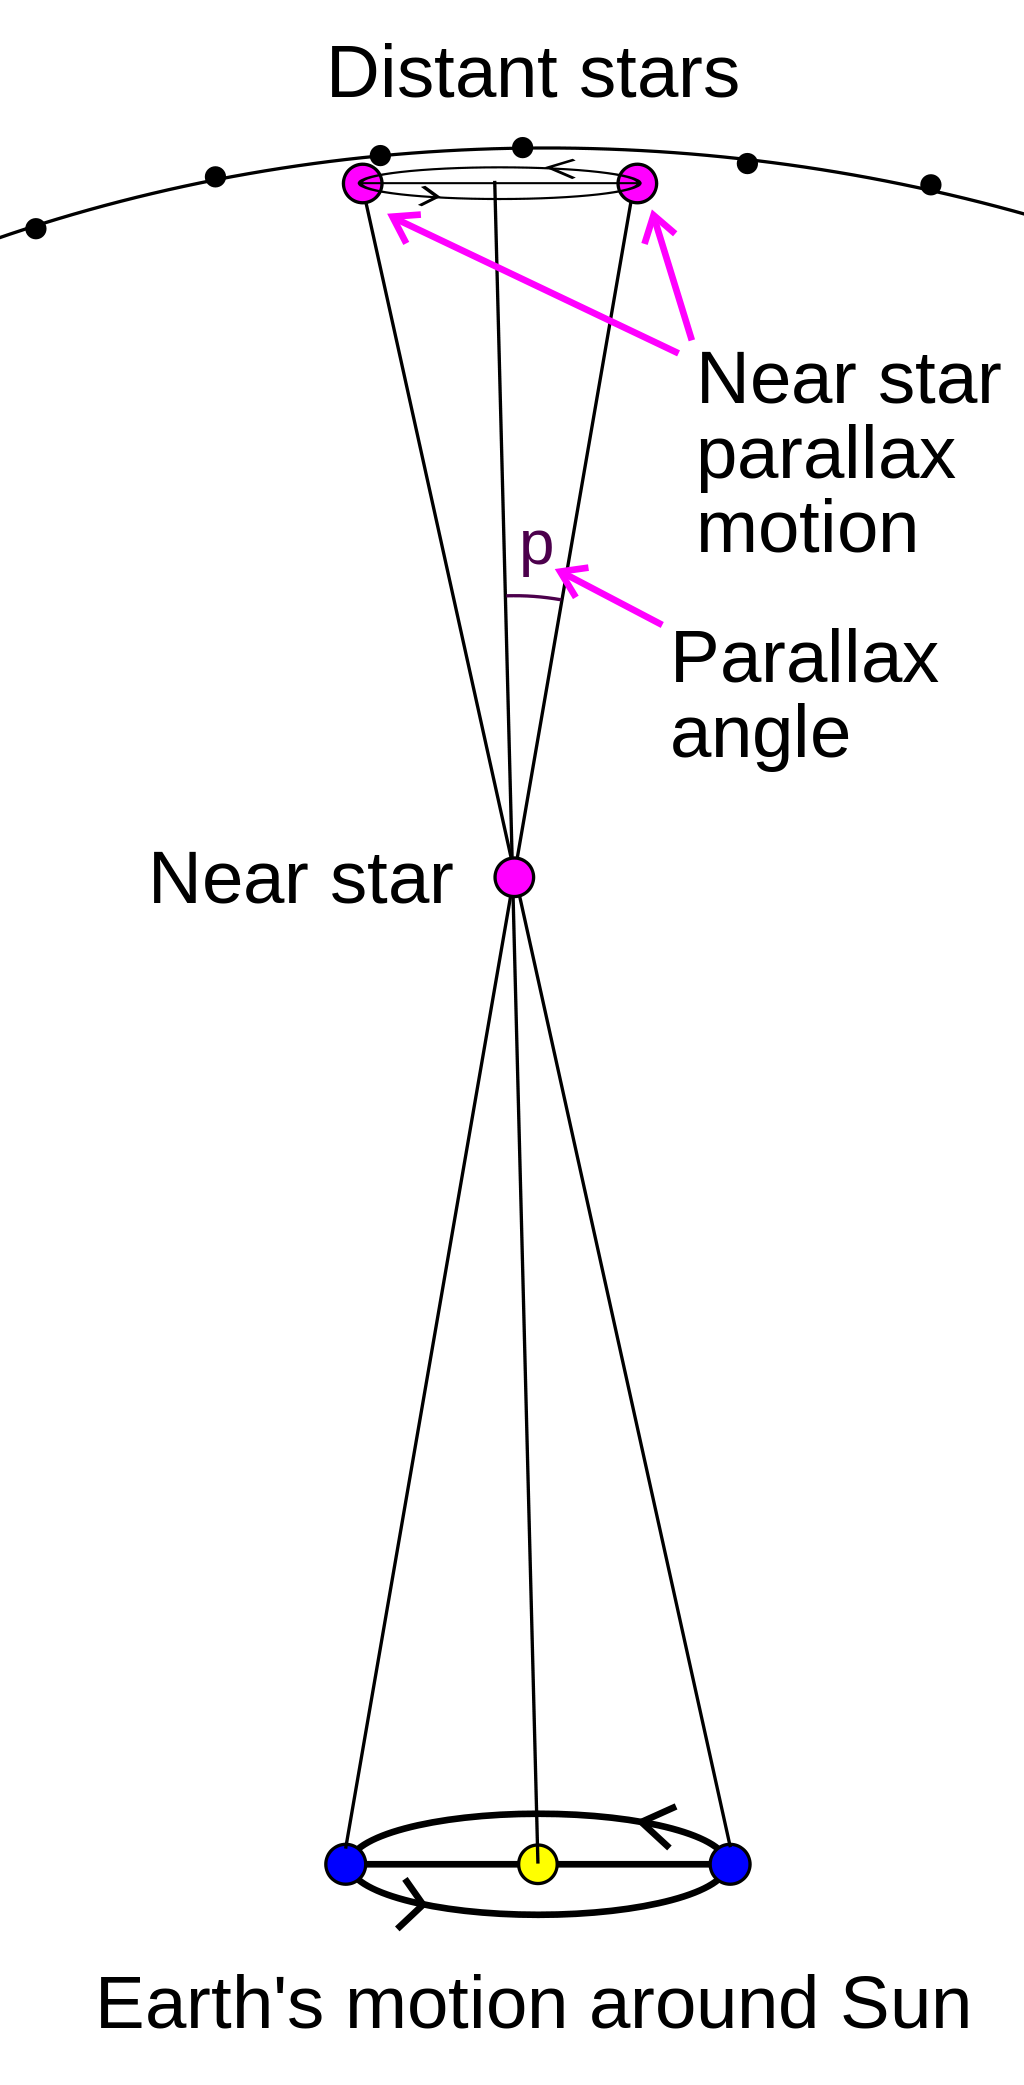
\includegraphics[width=0.6\columnwidth]{basicparallax.png}
			\caption{You have (almost certainly) seen this picture on wikipedia}
		\end{figure}
	\end{column}
\end{columns}

\end{frame}

\begin{frame}{Scanning Law }
\begin{columns}
\begin{column}{0.5\columnwidth}
		\begin{figure}
			\includegraphics[width=\columnwidth]{scanninglaw.png}
			\caption{Gaia Scan illustration\cite{collaborationGaia2016}}
		\end{figure}
\end{column}
\begin{column}{0.5\columnwidth}
		\begin{figure}
			\includegraphics[width=\columnwidth]{gaiaccd.png}
			\caption{Gaia CCD schematic\cite{collaborationGaia2016}}
		\end{figure}
\end{column}
\end{columns}

\end{frame}

\begin{frame}{Astrometric Solutions}

		\begin{figure}
			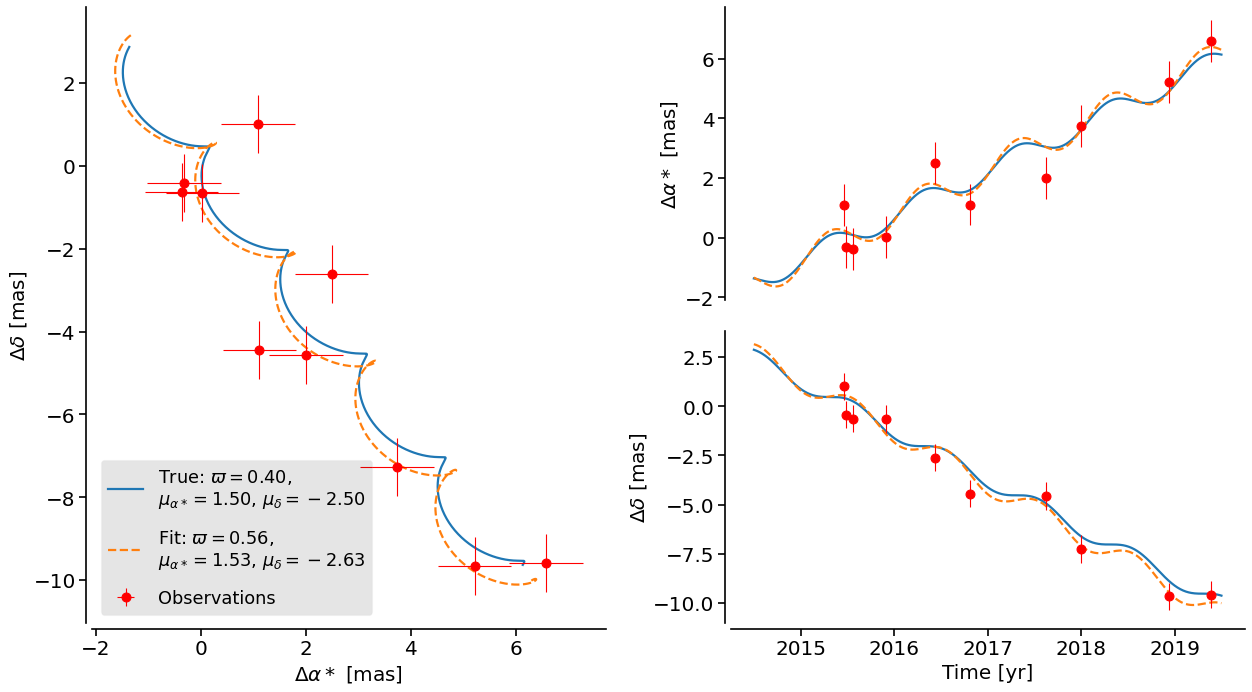
\includegraphics[width=\columnwidth]{astrometric-good.png}
			\caption{Figure generated from code in\cite{luriGaia2018}}
		\end{figure}

\end{frame}


\begin{frame}{Astrometric Solutions}

\center
\Huge What could possibly go wrong?
\end{frame}

\begin{frame}{What could possibly go wrong?}

\begin{columns}
\begin{column}{0.4\columnwidth}
\large Wrong assumptions
\normalsize
	\begin{itemize}
	\item Source Identification
	\item Source motion is linear
	\item Curve has a good fit
	\end{itemize}	
\vspace{10pt}
\large Causes
\normalsize
	\begin{itemize}
	\item Dim sources
	\item Bright sources
	\item Fast sources
	\item Slow sources
	\item Crowded fields
	\item Multiple star sources
	\item Variable sources
	\item Gravitational lensing
	\item Dark Companions
	\end{itemize}
\end{column}
\begin{column}{0.6\columnwidth}
\center
\large Spurious Astrometric Solutions
\normalsize
		\begin{figure}
			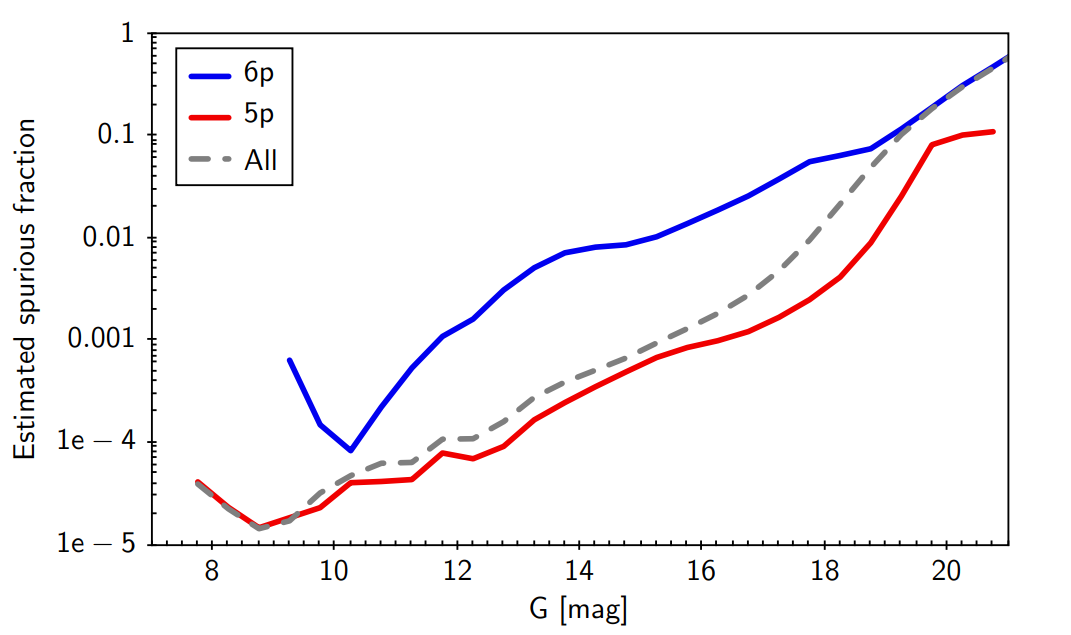
\includegraphics[width=\columnwidth]{spuriousfraction.png}
			\caption{Fraction of Spurious Astrometric solutions \cite{fabriciusGaia2021}}
		\end{figure}\end{column}
\end{columns}
\end{frame}

\begin{frame}{Bad Curve Fit}

		\begin{figure}
			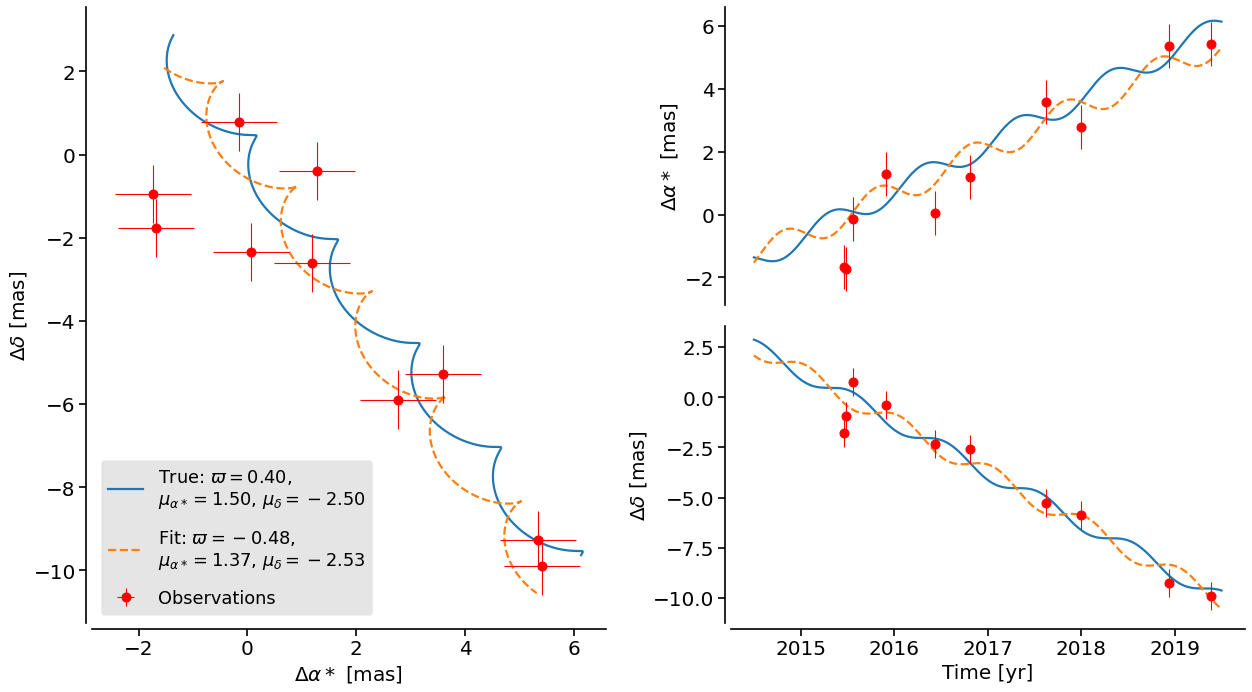
\includegraphics[width=\columnwidth]{astrometric-bad.png}
			\caption{Figure generated from code in \cite{luriGaia2018}}
		\end{figure}

\end{frame}

\begin{frame}{Parallax SNR}
		\begin{figure}
			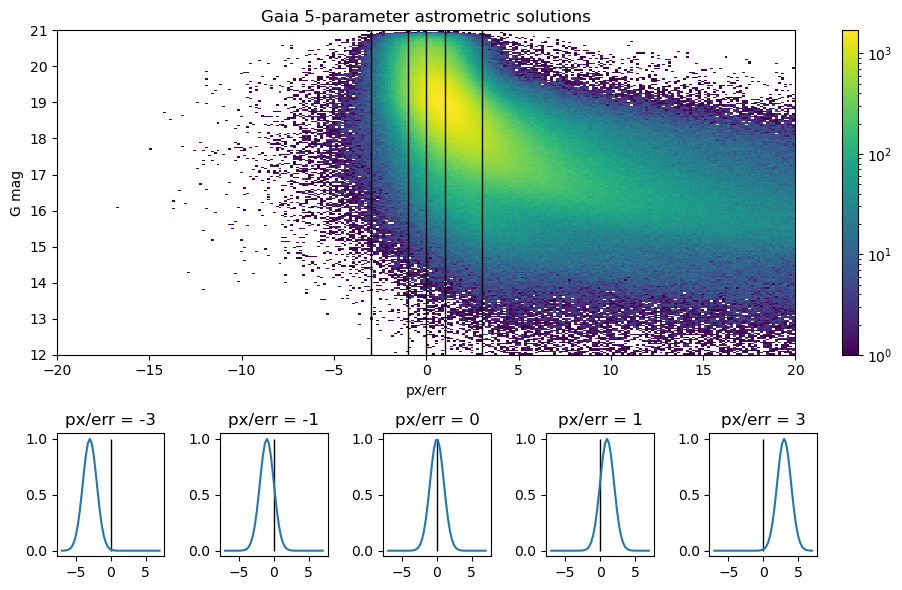
\includegraphics[width=\columnwidth]{poe_map.png}
			\caption{Data from \cite{collaborationGaia2022}\cite{collaborationGaia2016}}
		\end{figure}
\end{frame}

\begin{frame}{Bailer-Jones and Bayesian Inference}

\Large

Geometric: $P^*(r | \omega, \sigma_\omega, p) = P(r | p) P(\omega | r, \sigma_\omega)  $\\
\vspace{10pt}
Photogeometric: $P^*(r | \omega, \sigma_\omega, p, G, c) = P(Q_G | c, p) P(r | p) P(\omega | r, \sigma_\omega) $

\vspace{10pt}
\normalsize
\begin{itemize}
\item Likelihood: $P(\omega | r, \sigma_\omega)$ Probability you measure this parallax given a distance and error bars
\item Distance Prior: $P(r | p)$ Probability of distance given sky location from, Galaxy model fit to Gaia DR3 Simulated Galaxy\cite{bailer-jonesEstimating2021}\
\item Photometric prior $P(Q_G(r) | c, p)$ Probability you measure $Q_G = G - 5 log_10(r) + 5$ given the color and sky location\cite{bailer-jonesEstimating2021}\
\item To use: \texttt{...JOIN external.gaiaedr3\_distance as d USING (source\_id)...}
\item Parallax-only method with limited assumptions (unlike GSP-Phot)
\end{itemize}


\end{frame}

\begin{frame}{How well does this work?}
		\begin{figure}
			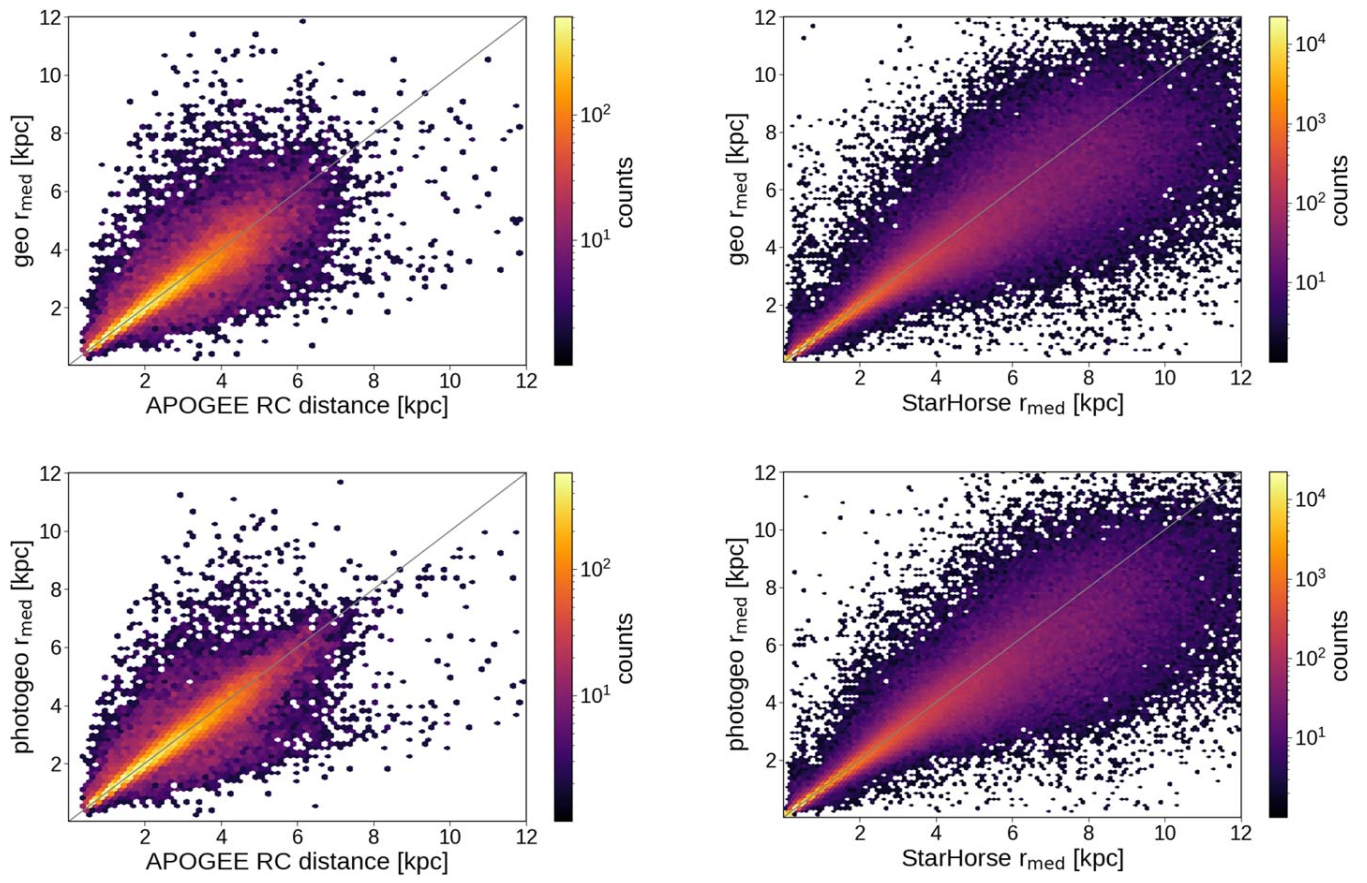
\includegraphics[width=0.8\columnwidth]{bailerjonesverification.png}
			\caption{Comparison of Bailer Jones distances to other methods \cite{bailer-jonesEstimating2021}}
		\end{figure}
		\begin{itemize}
			\item Around 6 kpc you start to see difference in prior coming out
			\item Hard to test a distance measure
		\end{itemize}
\end{frame}

\begin{frame}{DR4 makes it better?}
\begin{columns}
\begin{column}{0.5\columnwidth}
		\begin{figure}
			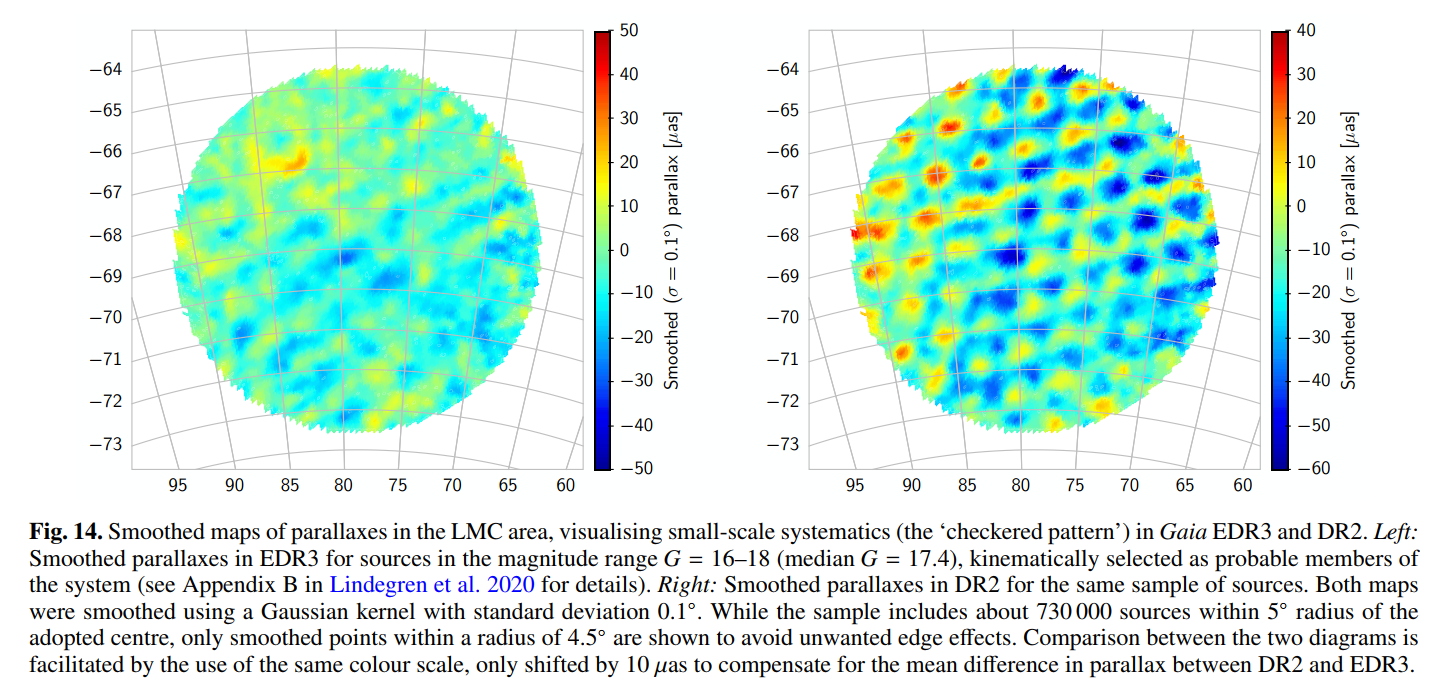
\includegraphics[width=\columnwidth]{lmcDR2vsDR3.png}
			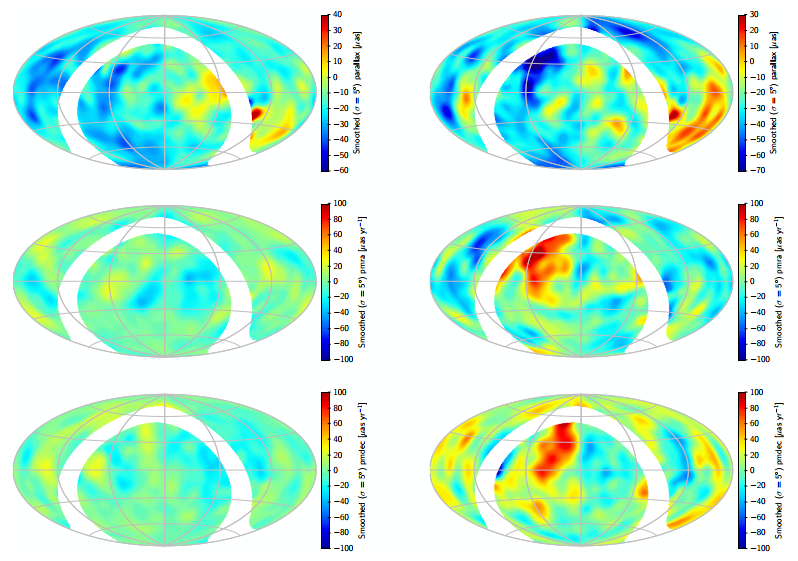
\includegraphics[width=\columnwidth]{quasar.png}
			\caption{Comparison of DR2 and EDR3 from \cite{lindegrenGaia2021a}}
		\end{figure}
\end{column}
\begin{column}{0.5\columnwidth}
		\begin{figure}
			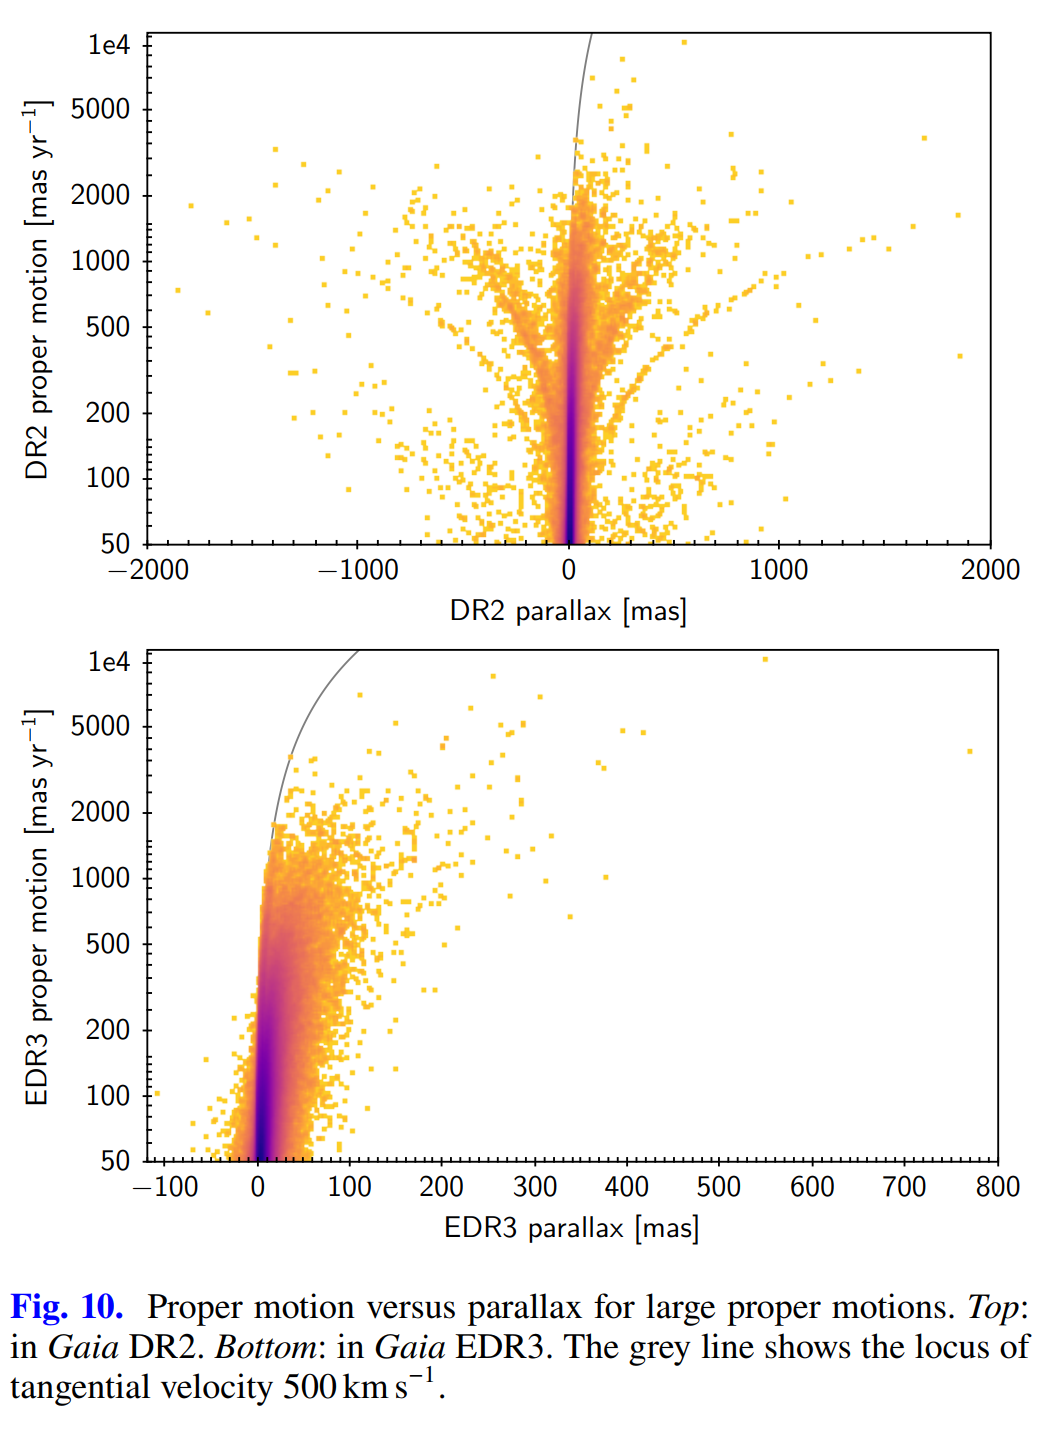
\includegraphics[width=\columnwidth]{parallaxvspropermotiondr2edr3.png}
			\caption{Figure from \cite{fabriciusGaia2021}}
		\end{figure}
\end{column}
\end{columns}
\end{frame}

\begin{frame}{Microlensing}
\begin{columns}
\begin{column}{0.5\columnwidth}
		\begin{figure}
			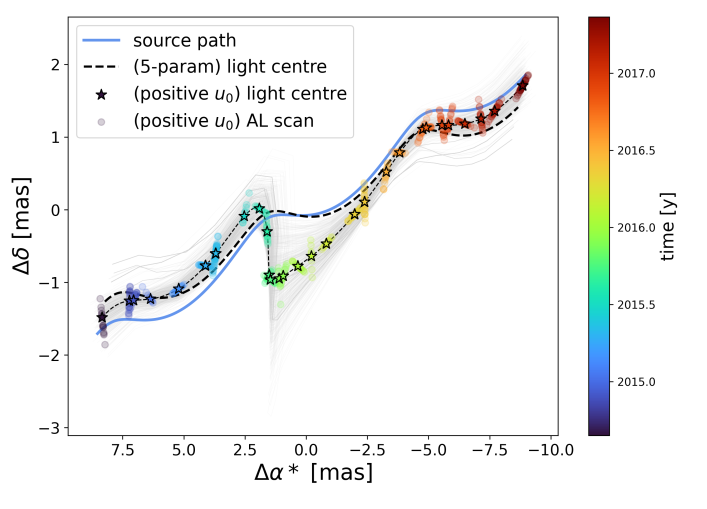
\includegraphics[width=\columnwidth]{microlensingpath.png}
			\caption{Figure from \cite{jablonskaThere2022}}
		\end{figure}
\end{column}
\begin{column}{0.5\columnwidth}
		\begin{figure}
			\includegraphics[width=\columnwidth]{microlensingsimMD.png}
			\includegraphics[width=\columnwidth]{microlensingsimTheta.png}
			\caption{Figure from \cite{jablonskaThere2022}}
		\end{figure}
\end{column}
\end{columns}

\end{frame}


\begin{frame}{References}
\printbibliography
\end{frame}

%\appendix
% Place to put non-numbered slides to answer expected questions

\end{document}


